In letteratura il problema affrontato in questa tesi è stato toccato da diversi contributi. In questo capitolo si illustrano due articoli molto correlati al lavoro qui presentato. Uno dei primi studi che ha riguardato il livello di privacy leakage contenuto nei mesaggi di testo divulgati in rete e più nello specifico su quelli divulgati su Twitter, viene condotto da Mao et al.~\cite{looseTweets}. In questo lavoro i ricercatori hanno cercato di categorizzare la natura dei leak nelle seguenti categorie:
\begin{itemize}
    \item leak provenienti da tweet di utenti in stato di ebrezza
    \item leak provenienti da tweet che rivelano i piani vacanze degli utenti
    \item leak provenienti da tweet che rivelano le informazioni mediche degli utenti
\end{itemize}
Per categorizzare la natura dei tweet verrà realizzato un classificatore in grado di rilevare i tweet affetti da leakage e infine viene effettuato uno studio comparativo per vedere quali argomenti sensibili vengono trattati in diverse nazioni.

La metodologia utilizzata da Mao et al.~\cite{looseTweets} per raggiungere i proprio obiettivi è la seguente
Inizialmente è stato realizzato un dataset contente i tweet presi dalla stream di Twitter nel periodo che va da gennaio a settembre 2010, una volta raccolti i tweet nel dataset questo è stato filtrato eliminando dal dataset di partenza i tweet che non contenevano le parole più ricorrenti trattate nelle categorie sopracitate. 

Utilizzando naive Bayes e SVM viene relizzato un classificatore in grado di rilevare la presenza di un leak in un tweet. Grazie ad esso è stato possibile effettuare una analisi comparativa per vedere quali argomenti vengono trattati principalmente nei testi affetti da leakage. I risultati sono i seguenti: in Figura~\ref{fig:res-ebbrezza} si mostrano i principali argomenti trattati nei tweet affetti da leak. Si nota come il 25\% riguardi "comportamenti irrispettosi".
\begin{figure}[h!t]
    \centering
    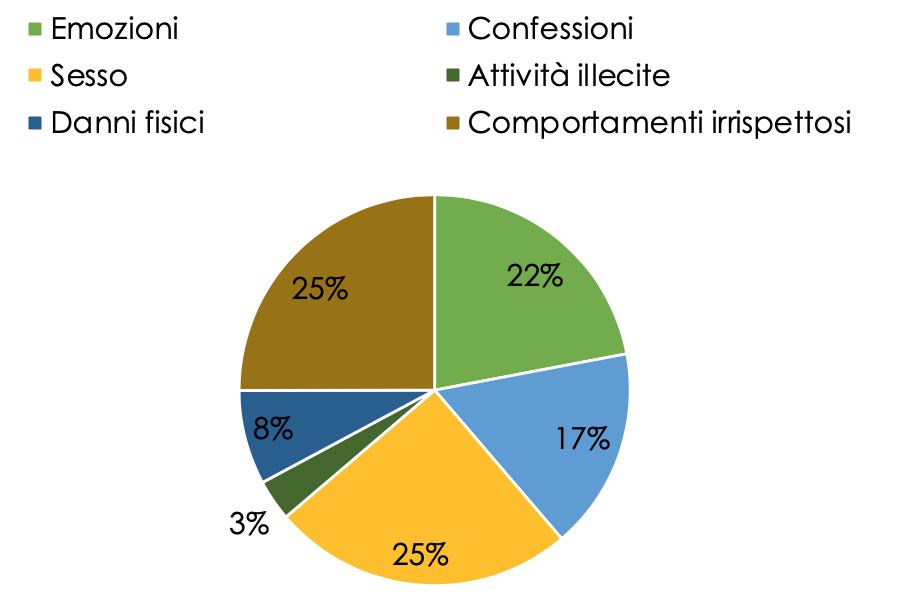
\includegraphics[width=15cm]{Figure/related_work/ebbrezza.png}
    \caption{argomenti trattati nei tweet fatti da utenti in stato di ebbrezza. Dati estrapolati da\cite{looseTweets}}
    \label{fig:res-ebbrezza}
\end{figure}
\FloatBarrier

In Figura~\ref{fig:res-patologie} si mostrano le patologie di cui maggiormente si parla nei tweet affetti da leak. Notiamo come, nel campione analizzato, più del 60\% dei tweet che trattano di salute vertano su \quotes{cancro}.

\begin{figure}[h!t]
    \centering
    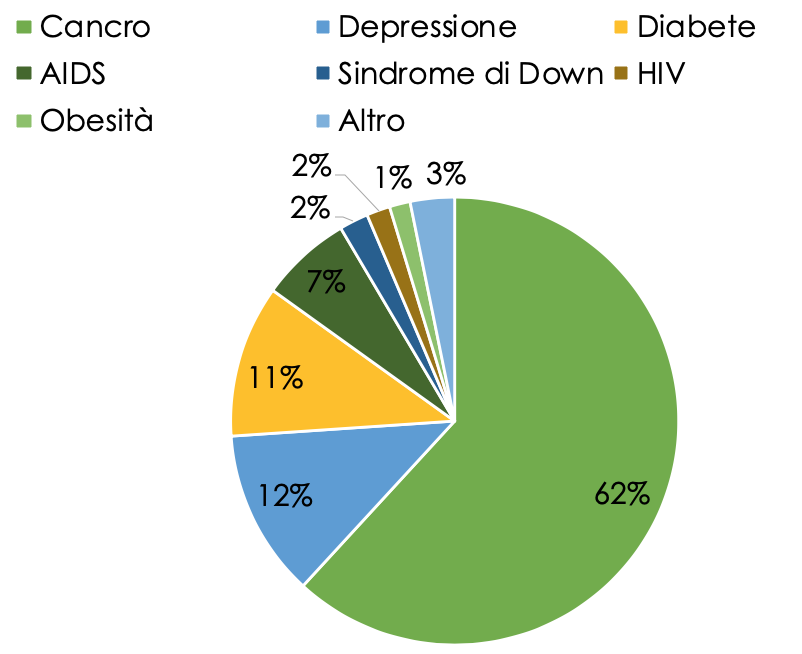
\includegraphics[width=15cm]{Figure/related_work/patologie.png}
    \caption{patologie contenute nei tweet che parlano di salute. Dati estrapolati da\cite{looseTweets}}
    \label{fig:res-patologie}
\end{figure}
\FloatBarrier

Infine i ricercatori hanno voluto effettuare una analisi comparativa andando a vedere quali patologie venivano trattate nei tweet riguardanti la categoria salute in tre diverse nazioni (Figura~\ref{fig:res-patologie-nazioni}). In tutte le nazioni considerate, USA, UK, Singapore la patologia più discussa è sempre il \quotes{cancro}.

\begin{figure}[h!t]
    \centering
    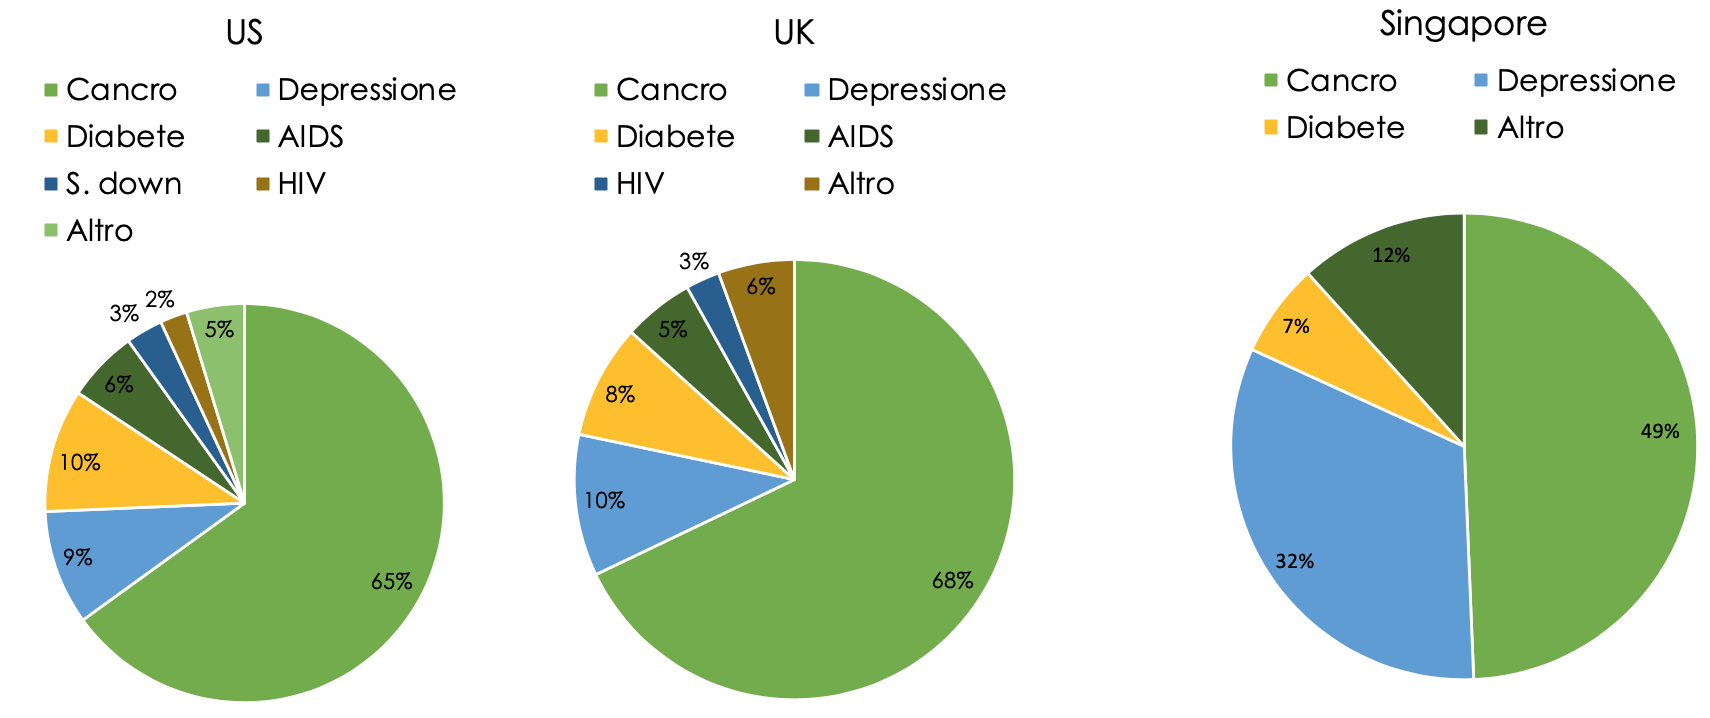
\includegraphics[width=15cm]{Figure/related_work/nazioni.png}
    \caption{patologie contenute nei tweet che parlano di salute. Dati estrapolati da\cite{looseTweets}}
    \label{fig:res-patologie-nazioni}
\end{figure}
\FloatBarrier


Fra le limitazioni di questo studio troviamo: (a) il modello realizzato non viene integrato in un tool, e/o messo a disposizione degli utenti finali, (b) la selezione dei testi che possono appartenere ad una categoria viene effettuata sulla base di keyword (non si tiene conto della semantica).

Nel lavoro di Mao et al.\cite{looseTweet} vengono per la prima volta individuate delle categorie di dati che si ritengono sensibili, alcune di queste categorie saranno presenti anche in studi successivi. Come nello studio di Qiaozhi et al.\cite{dontTweetThis} dove i ricercatori hanno proposto un modello quantitativo consapevole del contesto per la valutazione delle informazioni sensibili, andando così a definire una misura della sensibilità di un contenuto il \textbf{privscore}. Questo studio analizza i tweet che appartengono ad alcune categorie sensibili presenti anche in\cite{looseTweet} come i tweet che rivelano informazioni mediche e i tweet che parlano di droga e alcol, e ne aggiunge anche altre quali tweet che parlano di politica, oscenità, razzismo e informazioni personali o familiari.

In questo studio vengono proposti diversi tipi di \textbf{privscore}:
\begin{itemize}
    \item \textbf{Contex-free}: privscore che tiene conto della sensibilità del testo basandosi solo ed esclusivamente sul contenuto testuale
    \item \textbf{Contex-aware}: privscore che tiene conto del contesto in cui viene scritto un contenuto. Questo score integrato con il Context-free privscore ci consente di capire l’influenza sociale sulla percezione della privacy
    \item \textbf{Personalized}: privscore associato ad una frase conoscendo la percezione della privacy che ha l'utente che la sta scrivendo
    \item \textbf{Personalized Contex-Aware}: privscore associato ad una frase tenendo conto del contesto in cui essa viene scritta e della percezione di privacy che ha l'utente
\end{itemize}

Per realizzare un modello quantitativo consapevole del contesto per la valutazione delle informazioni sensibili i ricercatori hanno usato uno \quotes{Urban dictionary} contenente le parole più utilizzate nelle diverse categorie al fine di selezionare solo i tweet che contenessoro parole presenti nello \quotes{Urban Dictionary}. Così facendo è stato realizzato un dataset composta da 8079 tweet, in seguito tutti questi tweet sono stati etichettati con un valore che va da 1 a 5 (1 non sensibile 5 molto sensibile) dagli Amazon Turker(AMT).\footnote{https://www.mturk.com/}


\begin{figure}[h!t]
    \centering
    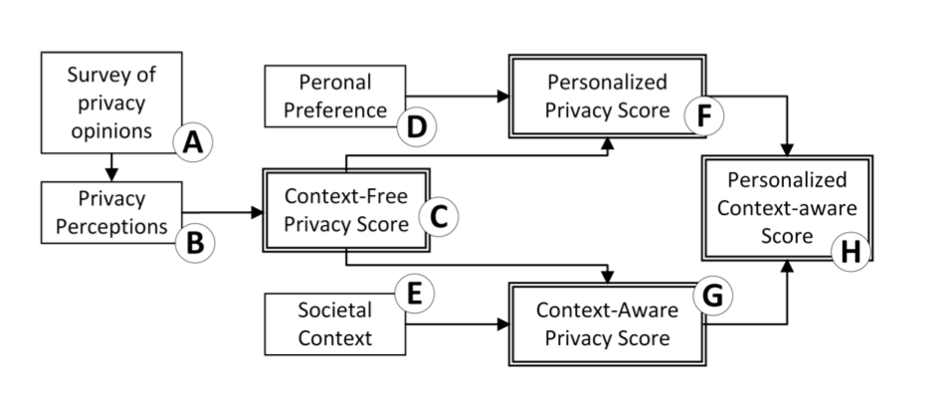
\includegraphics[width=15cm]{Figure/related_work/mtd-dontTweet.png}
    \caption{metodologia applicata per realizzare i vari privscore. Dati estrapolati da\cite{dontTweetThis}}
    \label{fig:mtd-dontTweetThis}
\end{figure}
\FloatBarrier

In Figura \ref{fig:mtd-dontTweetThis} vi è rappresentata la metodologia seguita in \cite{dontTweetThis}.

\begin{enumerate}
\item [A.]ai Turker è stato sottomesso un questionario per capire le loro opinioni sui dati sensibili
\item [B.]le risposte del questionario sono state analizzate per capire la percezione della privacy
\item [C.]in base ai risultati ottenuti viene sviluppato un modello di deep learning con word embedding per sviluppare il contex-free Priv Score
\item [D.]Viene analizzata la storia dei tweet fatti dall’utente per capire le sue preferenze in termini di privacy
\item [E.]Analisi del contesto sociale utilizzando il volume, la durata e la rilevanza di un trend topic. 
\item [F.]in base all' analisi fatta al punto D viene sviluppato un nuovo modello che integra le preferenze in termini di privacy dell'utente con il contex-free privscore
\item [G.]Il volume e la rilevanza dei trend topic è stata integrata con il context-free privscore al fine di mostrare la percezione della privacy da parte della società
\item [H.]Eventualmente gli studiosi svilupperanno un modello in grado di integrare il risultato del modello Personalized Privacy Score con il risultato del modello Context-aware Privacy Score al fine di realizzare un modello per il Personalized Context-aware score. Ovvero un modello in grado di riconoscere un contenuto sensibile basandosi sulla percezione della privacy che ha la società ma che tiene anche conto della percezione della privacy che ha l'utente.

Fra le limitazioni di questo studio c'è il fatto che l'accuratezza dei vari modelli può essere aumentata aumentando la quantità di dati annotati. Purtroppo il modello è fine a se stesso in quanto esso non viene integrato in un tool utilizzabile per fare analisi Infine fra le limitazioni c'è anche il fatto che sono stati utilizzati gli Amazon Turker per il labeling
\end{enumerate}

\begin{comment}
Al fine di tutelare i dati che gli utenti condividono con il loro passaggio online il 25 maggio del 2018 è entrata in vigore la normativa europea sulla protezione dei dati personali meglio nota come regolamento GDPR.\footnote{\url{https://eur-lex.europa.eu/legal-content/EN/TXT/HTML/?uri=CELEX:32016R0679&from=EN\#d1e40-1-1}}
Questa normativa limita il commercio dei dati ma di certo non impedisce agli utenti di pubblicare su un OSN informazioni sensibili in maniera volontaria o involontaria su se stesso o, peggio ancora, su altri. A tal proposito Mao et al. \cite{looseTweets} hanno condotto uno studio quantitativo su Twitter, lo studio ha rivelato che nei tweet sono presenti molti dati personali non solo riguardanti l'autore del tweet ma anche di terzi. In seguito Aylin et al.\cite{privacyDetective} hanno cercato di capire quanto siano sensibili le informazioni contenute nei tweet attribuendo a questi un \textbf{privacy score}, esso poteva essere di tre tipi:
\begin{enumerate}
    \item il tweet non contiene informazioni private
    \item il tweet può contenere informazioni private
    \item il tweet contiene informazioni private
\end{enumerate}
Questo studio si è concluso con il 10.37\% dei tweet collezionati ha un privacy score di tipo 1, il 21.11\% di tipo e il restante 68.52\% è di tipo 3.
Infine Qiaozhi et al. \cite{dontTweetThis} hanno cercato di fornire un' ulteriore misura della sensibilità presente nei vari tweet raccolti, le misure che hanno fornito sono i \textbf{privscore} essi si dividono in tre categorie
\begin{enumerate}
    \item liberi da contesto, un tweet che contiene un dato sensibile
    \item consapevoli del contesto, a seconda del contesto scritto nel tweet un dato può essere sensibile o meno
    \item personalizzati, a seconda della cronologia dei tweet fatti da un utente un dato può essere sensibile o meno
\end{enumerate}
\end{comment}